\documentclass[journal,12pt,twocolumn]{IEEEtran}

\usepackage{setspace}
\usepackage{gensymb}
\singlespacing
\usepackage[cmex10]{amsmath}

\usepackage{amsthm}

\usepackage{mathrsfs}
\usepackage{txfonts}
\usepackage{stfloats}
\usepackage{bm}
\usepackage{cite}
\usepackage{cases}
\usepackage{subfig}

\usepackage{longtable}
\usepackage{multirow}

\usepackage{enumitem}
\usepackage{mathtools}
\usepackage{steinmetz}
\usepackage{tikz}
\usepackage{circuitikz}
\usepackage{verbatim}
\usepackage{tfrupee}
\usepackage[breaklinks=true]{hyperref}
\usepackage{graphicx}
\usepackage{tkz-euclide}

\usetikzlibrary{calc,math}
\usepackage{listings}
    \usepackage{color}                                            %%
    \usepackage{array}                                            %%
    \usepackage{longtable}                                        %%
    \usepackage{calc}                                             %%
    \usepackage{multirow}                                         %%
    \usepackage{hhline}                                           %%
    \usepackage{ifthen}                                           %%
    \usepackage{lscape}     
\usepackage{multicol}
\usepackage{chngcntr}

\DeclareMathOperator*{\Res}{Res}

\renewcommand\thesection{\arabic{section}}
\renewcommand\thesubsection{\thesection.\arabic{subsection}}
\renewcommand\thesubsubsection{\thesubsection.\arabic{subsubsection}}

\renewcommand\thesectiondis{\arabic{section}}
\renewcommand\thesubsectiondis{\thesectiondis.\arabic{subsection}}
\renewcommand\thesubsubsectiondis{\thesubsectiondis.\arabic{subsubsection}}

\newtheorem{theorem}{Theorem}
\hyphenation{op-tical net-works semi-conduc-tor}
\def\inputGnumericTable{}                                 %%

\lstset{
%language=C,
frame=single, 
breaklines=true,
columns=fullflexible
}
\begin{document}

\newcommand{\BEQA}{\begin{eqnarray}}
\newcommand{\EEQA}{\end{eqnarray}}
\newcommand{\define}{\stackrel{\triangle}{=}}
\bibliographystyle{IEEEtran}
\raggedbottom
\setlength{\parindent}{0pt}
\providecommand{\mbf}{\mathbf}
\providecommand{\pr}[1]{\ensuremath{\Pr\left(#1\right)}}
\providecommand{\qfunc}[1]{\ensuremath{Q\left(#1\right)}}
\providecommand{\sbrak}[1]{\ensuremath{{}\left[#1\right]}}
\providecommand{\lsbrak}[1]{\ensuremath{{}\left[#1\right.}}
\providecommand{\rsbrak}[1]{\ensuremath{{}\left.#1\right]}}
\providecommand{\brak}[1]{\ensuremath{\left(#1\right)}}
\providecommand{\lbrak}[1]{\ensuremath{\left(#1\right.}}
\providecommand{\rbrak}[1]{\ensuremath{\left.#1\right)}}
\providecommand{\cbrak}[1]{\ensuremath{\left\{#1\right\}}}
\providecommand{\lcbrak}[1]{\ensuremath{\left\{#1\right.}}
\providecommand{\rcbrak}[1]{\ensuremath{\left.#1\right\}}}
\theoremstyle{remark}
\newtheorem{rem}{Remark}
\newcommand{\sgn}{\mathop{\mathrm{sgn}}}
\providecommand{\abs}[1]{\vert#1\vert}
\providecommand{\res}[1]{\Res\displaylimits_{#1}} 
\providecommand{\norm}[1]{\lVert#1\rVert}
%\providecommand{\norm}[1]{\lVert#1\rVert}
\providecommand{\mtx}[1]{\mathbf{#1}}
\providecommand{\mean}[1]{E[ #1 ]}
\providecommand{\fourier}{\overset{\mathcal{F}}{ \rightleftharpoons}}
%\providecommand{\hilbert}{\overset{\mathcal{H}}{ \rightleftharpoons}}
\providecommand{\system}{\overset{\mathcal{H}}{ \longleftrightarrow}}
	%\newcommand{\solution}[2]{\textbf{Solution:}{#1}}
\newcommand{\solution}{\noindent \textbf{Solution: }}
\newcommand{\cosec}{\,\text{cosec}\,}
\providecommand{\dec}[2]{\ensuremath{\overset{#1}{\underset{#2}{\gtrless}}}}
\newcommand{\myvec}[1]{\ensuremath{\begin{pmatrix}#1\end{pmatrix}}}
\newcommand{\mydet}[1]{\ensuremath{\begin{vmatrix}#1\end{vmatrix}}}
\numberwithin{equation}{subsection}
\makeatletter
\@addtoreset{figure}{problem}
\makeatother
\let\StandardTheFigure\thefigure
\let\vec\mathbf
\renewcommand{\thefigure}{\theproblem}
\def\putbox#1#2#3{\makebox[0in][l]{\makebox[#1][l]{}\raisebox{\baselineskip}[0in][0in]{\raisebox{#2}[0in][0in]{#3}}}}
     \def\rightbox#1{\makebox[0in][r]{#1}}
     \def\centbox#1{\makebox[0in]{#1}}
     \def\topbox#1{\raisebox{-\baselineskip}[0in][0in]{#1}}
     \def\midbox#1{\raisebox{-0.5\baselineskip}[0in][0in]{#1}}
\vspace{3cm}
\title{GATE Assignment}
\author{Digjoy Nandi - AI20BTECH11007}
\maketitle
\newpage
\bigskip
\renewcommand{\thefigure}{\theenumi}
\renewcommand{\thetable}{\theenumi}
Download all python codes from 
\begin{lstlisting}
https://github.com/Digjoy12/Signal-Processing/blob/main/Assignment_5/Codes/Code.py
\end{lstlisting}
%
and latex codes from 
%
\begin{lstlisting}
https://github.com/Digjoy12/Signal-Processing/blob/main/Assignment_5/main.tex
\end{lstlisting}
\section*{\textbf{Problem}}
\textbf{(Quadratic Forms Q2.67)} The line $\myvec{-m & 1}\vec{x} = 1$ is a tangent to the curve $y^2 = 4x$. Find the value of m. 
\section*{\textbf{Solution}}
Given equation,
\begin{equation}
    y^2 = 4x
\end{equation}
Comparing it with the standard equation,
\begin{equation}
    ax^2 + 2bxy + cy^2 + 2dx + 2cy + f = 0
\end{equation}
Here, 
$a = b = c = f = 0$, $d = -2$ and $c = 1$
\begin{equation}
    \therefore \vec{V} = \myvec{a & b \\ b & c} = \myvec{0 & 0 \\ 0 & 1} \label{0.0.3}
\end{equation}
\begin{equation}
    \therefore \vec{u} = \myvec{d \\ e} = \myvec{-2 \\ 0} \label{0.0.4}
\end{equation}
Now,
\begin{equation}
   \abs{\vec{V}} = \begin{vmatrix}0 & 0\\ 0 & 1\end{vmatrix} = 0 
\end{equation}
$\implies$ the curve is a parabola. Now, finding
the eigen values corresponding to the $\vec{V}$.
\begin{align}
    \begin{vmatrix}\vec{V} - \lambda\vec{I}\end{vmatrix} &= 0\\
    \implies \begin{vmatrix}
    -\lambda & 0 \\ 0 & 1 - \lambda
    \end{vmatrix} &= 0\\
    \implies -\lambda(1 - \lambda) &= 0
\end{align}
$\therefore$ $\lambda = 0$ or $\lambda = 1$\\
Calculating the eigen vectors corresponding to $\lambda$ = 0, 1 respectively,
\begin{equation}
    \vec{Vx} = \lambda\vec{x}
\end{equation}
\begin{align}
    \myvec{0 & 0 \\ 0 & 1}\vec{x} = 0 \implies& \vec{p_1} = \myvec{1 \\ 0}\\
    \myvec{-1 & 0 \\ 0 & 0}\vec{x} = 0 \implies& \vec{p_2} = \myvec{0 \\ 1}
\end{align}
Now by eigen decomposition on $\vec{V}$,
\begin{equation}
    \vec{V} = \vec{PDP^{T}} \label{0.0.12}
\end{equation}
where,
\begin{equation}
    \vec{P} = \myvec{\vec{p_1} & \vec{p_2}} = \myvec{1 & 0\\ 0 & 1}
\end{equation}
and,
\begin{equation}
    \vec{D} = \myvec{\lambda_1 & 0 \\ 0 & \lambda_2} = \myvec{0 & 0 \\ 0 & 1}
\end{equation}
Now, equation \eqref{0.0.12} becomes,
\begin{align}
    \vec{V} &= \myvec{1 & 0\\ 0 & 1}\myvec{0 & 0 \\ 0 & 1}\myvec{1 & 0\\ 0 & 1}\\
    &= \myvec{0 & 0 \\ 0 & 1}
\end{align}
The given line equation is
\begin{align}
    \myvec{-m & 1}\vec{x} = 1\\
    \implies -mx + y - 1 = 0 
\end{align}
The general straight line equation is of the form
\begin{equation}
    ax + by + c = 0
\end{equation}
The normal vector (\vec{n}) and direction (\vec{m}) are
given by,
\begin{align}
    \vec{n} = \myvec{a \\ b} = \myvec{-m \\ 1} \label{0.0.20}\\
    \vec{m} = \myvec{b \\ -a} = \myvec{1 \\ m}
\end{align}
Now, the equation for the point of contact for the parabola is given as,
\begin{equation}
    \myvec{\vec{u}^{T} + k\vec{n}^{T}\\\vec{V}}\vec{q} = \myvec{-f \\ k\vec{n}-\vec{u}} \label{0.0.22}
\end{equation}
where,
\begin{equation}
    k = \cfrac{\vec{p_1}^{T}\vec{u}}{\vec{p_1}^{T}\vec{n}} = \cfrac{\myvec{1 & 0}\myvec{-2 \\ 0}}{\myvec{1 & 0}\myvec{-m \\ 1}} = \cfrac{2}{m} \label{0.0.23}
\end{equation}
Hence, substituting the values of \eqref{0.0.3}, \eqref{0.0.4}, \eqref{0.0.20} and \eqref{0.0.23} in the equation \eqref{0.0.22}, we get
\begin{align}
    \myvec{\myvec{-2 & 0} + \cfrac{2}{m}\myvec{-m & 1} \\ 0 & 0 \\ 0 & 1}\vec{q} &= \myvec{0 \\ \cfrac{2}{m}\myvec{-m \\ 1}-\myvec{-2\\0}}\\
    \implies \myvec{-4 & \cfrac{2}{m}\\ 0 & 0 \\ 0 & 1}\vec{q} &= \myvec{0 \\ 0 \\ \cfrac{2}{m}}\label{0.0.25}
\end{align}
Solving for q by removing the zero row and representing \eqref{0.0.25} as augmented matrix and then converting the matrix to echelon form
\begin{align}
    \myvec{-4 & \cfrac{2}{m} & 0 \\ 0 & 1 & \cfrac{2}{m}} \xleftrightarrow{\text{$R_1$}\rightarrow{\text{$-\frac{1}{4}R_1$}}} \myvec{1 & \cfrac{-1}{2m} & 0 \\ 0 & 1 & \cfrac{2}{m}}\\
    \xleftrightarrow{\text{$R_2$}\rightarrow{\text{$R_{1}+\frac{1}{2m}R_2$}}}
    \myvec{1 & 0 & \cfrac{1}{m^2} \\ 0 & 1 & \cfrac{2}{m}} \label{0.0.27}
\end{align}
Hence from equation \eqref{0.0.27} it can be concluded that the point of contact is,
\begin{equation}
    \vec{q} = \myvec{\cfrac{1}{m^2} \\ \cfrac{2}{m}}
\end{equation}
Now $\vec{q}$ is a point on the tangent. Hence, the equation of the line can be expressed as
\begin{equation}
    \vec{n}^{T}\vec{x} = c = 1
\end{equation}
where,
\begin{align}
    c = \vec{n}^{T}\vec{q} &= 1\\
    \implies \myvec{-m & 1}\myvec{\cfrac{1}{m^2} \\ \cfrac{2}{m}} &= 1\\
    \implies \cfrac{-1}{m} + \cfrac{2}{m} &= 1\\
    \implies \cfrac{1}{m} &= 1\\
    \implies m &= 1
\end{align}
Hence, the line $\myvec{-m & 1}\vec{x} = 1$ is a tangent to the curve $y^2 = 4x$ when \textbf{m = 1}.
\begin{figure}[!ht]
\centering
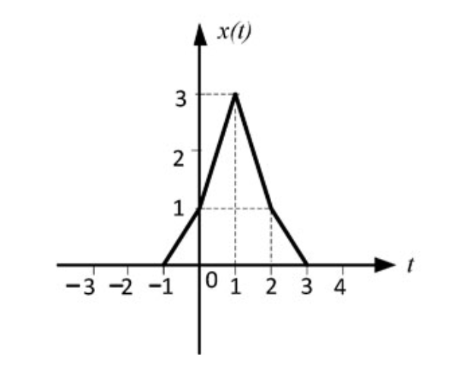
\includegraphics[width=\columnwidth]{plot.png}
\end{figure}
\end{document}

